\chapter{Objetivos}

Una vez situado el Trabajo Fin de Grado en su contexto vamos a presentar los objetivos concretos que nos marcamos para la realización del mismo.


\section{Objetivos}

Como objetivo global nos proponemos teleoperar un drone desde dispositivos móviles cómo teléfonos o tabletas utilizando tecnologías web de ultima generación. Este objetivo se ha desglosado en tres subobjetivos concretos que explicamos a continuación.\\

Como escenario nos encontramos con un drone que irá a bordo del drone, y una navegador en una máquina remota. Durante toda la memoria nos referiremos como ordenador local, par local o navegador local al dispositivo que usaremos para conectarnos al cuadricóptero y el cuál deberá ir a bordo del drone, y ordenador remoto, par remoto o navegador remoto al ordenador desde el cuál teleoperaremos el vehículo.\\

\begin{itemize}


\item \emph{\textbf{Conexión local}}: Como primer subobjetivo tenemos que desarrollar una conexión directa del navegador local con el \emph{hardware} del drone. Esta conexión tiene que ser bidireccional, ya que tenemos que acceder a los sensores y actuadores del drone, así como a su cámara, pero también es necesario mandarle órdenes de movimiento.\\

Como requisito fundamental para esta conexión con el servidor de los actuadores y sensores a bordo es que tiene que ser en tiempo real y que sea lo suficientemente fluida y ligera como para que no introduzca ningún tipo de retardo.\\


\item \emph{\textbf{Conexión multimedia entre navegadores}}: El segundo punto con el que nos enfrentamos es utilizar una tecnología web moderna y actual con la que poder teleoperar el drone. Esta tecnología tiene que ser lo suficientemente versátil como para poder implementarla en nuestro proyecto. Por otro lado, al igual que la conexión local, tiene que ser bidireccional, poder transportar audio, vídeo y datos genéricos e introducir el mínimo retraso en la comunicación posible para tener una experiencia positiva y controlada del vuelo del drone.\\

Esta conexión deberá realizarse entre el ordenador local y un segundo ordenador, que será desde el que el usuario podrá teleoperar el vehículo.\\


\item \emph{\textbf{Interfaz de usuario amigable}}: Uno de los subobjetivos es desarrollar una interfaz web de usuario clara, que nos muestre de una manera lo más realista, clara y concisa posible los datos recogidos de los sensores del drone y la cámara para permitirnos conocer el estado de vuelo del drone en cada momento: altitud, inclinación, velocidad...\\

Esta interfaz deberá permitirnos el manejo del cuadricóptero de la forma mas realista y similar posible a los sistemas de control de drones que hemos hablado en el capítulo \ref{cap:controldrones}. Para que la satisfacción de vuelo sea satisfactoria la interfaz tiene que tener unos controles de movimiento que sean sencillos, simples e intuitivos.\\

\end{itemize}


\section{Metodología y plan de trabajo}

La realización de un proyecto requiere una metodología que establezca las pautas a seguir y la planificación de las tareas que se deben llevar a cabo para cumplir los objetivos. Hemos escogido el modelo de \emph{desarrollo en espiral}, ya que es un modelo ampliamente usado en la ingeniería de \emph{software}. Este modelo define una serie de ciclos que se repiten en un bucle hasta el final del proyecto, dividiéndolo en varias subtareas más sencillas y estableciendo puntos de control al final de cada iteración en los que se evalúa el trabajo realizado y se enfocan las nuevas tareas para continuar.\\

Esta metodología recibe su nombre por la forma de espiral que tiene su representación gráfica o diagrama de flujo, que podemos ver en la figura \ref{fig:planificacion_espiral}. En cada iteración se llevan a cabo las siguientes actividades:

\begin{itemize}
 \item \textbf{Determinar los objetivos}, dividir en subobjetivos y fijar requisitos.
 \item \textbf{Analizar los riesgos} y factores que impidan o dificulten el trabajo y las consecuencias negativas que este
 pueda ocasionar.
 \item \textbf{Desarrollar} las tareas para lograr los objetivos según los requisitos especificados.
 \item \textbf{Planificar} las próximas fases tras evaluar el transcurso del proyecto.
\end{itemize}

\begin{figure}[htb]
\centering
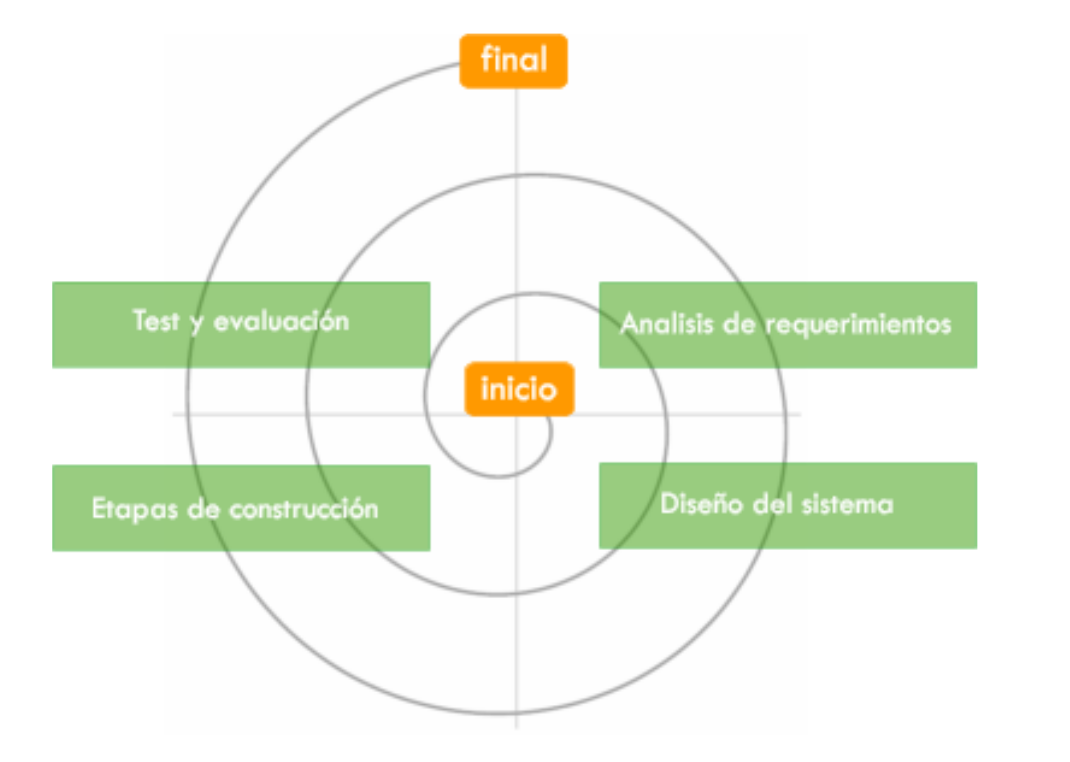
\includegraphics[width=0.9\textwidth]{espiral}
\caption{Esquema general del desarrollo del proyecto.}
\label{fig:planificacion_espiral}
\end{figure}

Durante el ciclo de vida del proyecto se han hecho reuniones periódicas con el tutor. En ellas se evaluaban los avances logrados y se marcaba la hoja de ruta a tomar para los siguientes días de desarrollo. Si los puntos marcados en sesiones anteriores no se habían finalizado se ampliaba el plazo o se intentaba buscar otra manera de avance.\\

Para facilitar el seguimiento del proyecto se ha utilizado de un mediawiki\footnote{http://jderobot.org/Irodmar-tfg} de JdeRobot en el que se iba actualizando cada avance que se lograba, con explicaciones y vídeos e imágenes. Para el código fuente se ha empleado un repositorio en la plataforma web de control de versiones GitHub\footnote{https://github.com/RoboticsURJC-students/2015-tfg-irodmar}.\\

El plan de trabajo para todo el proyecto se puede dividir en las siguientes etapas:

\begin{itemize}
\item \textbf{Familiarización con JdeRobot}: Primer contacto con esta plataforma y sus herramientas para conocer su funcionamiento.
\item \textbf{Aprendizaje de tecnologías web necesarias:} Conocer las tecnologías web que van a ser necesarias para el desarrollo del proyecto. Entre ellas se encuentra WebRTC, HTML5, CSS3, WebGL, ThreeJS, o jQuery. Primer contacto también con el \emph{middleware} ICE.
\item \textbf{Desarrollo de la conexión local:} Creación de toda la infraestructura necesaria para la interconexión entre el navegador local y el drone.
\item \textbf{Desarrollo conexión entre navegadores}: Desarrollo de la conexión remota que interconectará los dos pares.
\item \textbf{Desarrollo interfaz web de usuario}: Desarrollo de la interfaz amigable para teleoperar el drone.
\item \textbf{Experimentos}: Primero se realizan pruebas con el simulador, y cuando el código este suficientemente maduro se prueba con un drone real.
\end{itemize}






